\documentclass[12pt]{book}
\usepackage[a5paper]{geometry}

\usepackage[utf8]{inputenc}
\usepackage{tipa}
% \usepackage[german]{babel}
\usepackage{graphicx}

\setlength{\parindent}{1em}
%\setlength{\parskip}{1em}

\begin{document}
\begin{titlepage}

\author{Krizhanich Research Institute of Novoslovnica}
\title{%
	Novoslovnica \\
	\large Guide through a Slavic constructed language
\vfill
}
\date{2015-2019}

\end{titlepage}

\frontmatter
\maketitle
\tableofcontents
\mainmatter
\chapter{Phonology}

Every language has its own phonology. But do you know what phonology is?

Phonology - a branch of linguistics concerned with the systematic organization of sounds in the language.

Thus, phonology describes all the sounds that the language possesses. Sounds can be divided into different classes. One of the characteristics separating different sounds is the ability to pronounce them with an open vocal tract. You can notice that vowels (such as a, o, u in English) are able to be pronounced with open vocal tract, whereas consonants are pronounced with partly or completely closed vocal tract. So, let's discuss the sounds from the point of this classification.

However, firstly we should speak about the term allophone.

Allophone - one of a set of multiple possible spoken sounds or signs used to pronounce a single phoneme in a particular language.

Well, what is a phoneme? A phoneme is one of the units of sound that distinguish one word from another in a particular language. Simply put, it is such a sound (or a set of sounds) that do not influence the meaning of the word. 


\section{Vowels}

In the beginning of this paragraph I would like to write a description of a vowel.

Vowel - a sound produced with no constriction in the vocal tract.

With this information we can distinguish different types of vowels. The classification of vowels is based on two main factors:
What is the row of the sound
What is the height of the sound
Whether the vowel is rounded or not

The row is the position of the tongue when you pronounce a vowel. There are three main rows: front, central and back. When you pronounce a vowel at the front row, you move your tongue toward the teeth. The descriptions of central and back rows are similar - you move your tongue to the center or toward the larynx to pronounce them.

The height of the sound is a characteristic of tongue convexity and tension in your mouth. If it is positive, it means your tongue does not touches the palate nor bottom of the mouth, and the tip of your tongue is tense- or closed. If your tongue is flat and parallel to the bottom of your oral cavity, moreover, it lies on it - it is an open one. Between these two positions a middle position can be found.

The roundedness of the vowel is the amount of rounding in the lips during the articulation of a vowel. Vowels can be categorized as rounded and unrounded. Thus, to pronounce a rounded vowel you should round your lips. To pronounce an unrounded vowel, you should relax your lips during the articulation of a vowel.

Finally, we can talk about Novoslovnica phonology. Novoslovnica consists of 20 ordinary vowel phonemes. Among them there are seven closed vowels, three open vowels, ten middle vowels as well as seven front vowels, five center vowels and eight back vowels. On the table 1.1 you can see a chart position of the vowels in Novoslovnica.

\begin{table}[]
	\begin{tabular}{lllll}
		& Front & Center & Near-back & Back \\
		Close      &       &        &           &      \\
		Near-close &       &        &           &      \\
		Close-mid  &       &        &           &      \\
		Mid        &       &        &           &      \\
		Open-mid   &       &        &           &      \\
		Open       &       &        &           &     
	\end{tabular}
\end{table}

In this table you can also see different colors of the vowels. The green ones are for rounded vowels. Yellow ones are for unrounded vowels.

If you know Czech or Finnish, you might be concerned by the absence long vowels in this chart. It’s time to speak about allophones in Novoslovnica.

Novoslovnica has allophones of open and long vowels. This means that it does not matter how you pronounce a “modified” vowel - as a long one or as an open one - the meaning of the word will not change. To make this more clear, look at table 1.2.


\chapter{Orthography}

\begin{figure}
	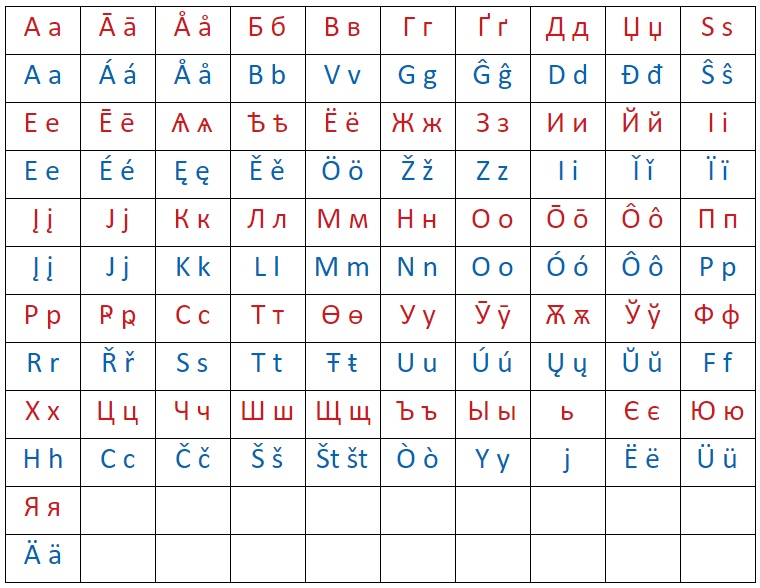
\includegraphics[width=\linewidth]{./sources/alphabet.jpg}
	\caption{Alphabet of Novoslovnica}
	\label{fig:alphabet}
\end{figure}

\section{Alphabet}

Let’s summarize what we have known about Novoslovnica phonology. Afterwards we will get the list of phonemes and allophones and their connections with Novoslovnica letters in the alphabet.

We have learned that Novoslovnica has 51 consonant sounds and 22 vowels. 13 consonants and 4 vowels are allophones among them. Hence, the amount of phonemes is (51-13) + (22 - 4) = 56 phonemes.

You should know that in Novoslovnica, soft and hard consonants do not differ in writing. That is because of the fact that by the combination of “consonant + vowel” we can always determinedly get what the consonant is like - hard or soft. With this information, the amount of letters needed is reduced to 49 \cite{nsl-alphabet}.

Nevertheless, let’s now look at the table with the alphabet list and see how Novoslovnica is written.

% \begin{table}
	\begin{longtable}{llllp{4em}p{6em}}
		No. & Char & Cyr & Phoneme & Allophone & Examples in English \\
		\endhead
		1 & A a & А а & \textipa{[a]} & & Ex\textbf{a}mple, p\textbf{a}st (British forms) \\
		2 & Ä ä & Я я & \textipa{[\ae]} &  & Cat, rat (American English) \\
		3 & Á á & Ā ā & \textipa{[a:]} & \textipa{[A]} & M\textbf{a}rk, p\textbf{a}rk \\
		4 & Å å & Å å & \textipa{[2]} & & C\textbf{u}t, w\textbf{o}nder \\
		5 & B b & Б б & \textipa{[b]} & \textipa{[bj]} & \textbf{B}etter, \textbf{b}ear \\
		6 & C c & Ц ц & \textipa{[\t{ts}]} & \textipa{[\t{ts}j]} & Tea, team (In some American or British dialects) \\
		7 & Č č & Ч ч & \textipa{[\t{tS}]} & \textipa{[\t{tC}], [\t{t\:s}]} & Cheese, check \\
		8 & D d & Д д & \textipa{[d]} & \textipa{[\textbardotlessj]} & Do, dinner \\
		9 & Đ đ & Џ, џ & \textipa{[\t{\:d\:z}]} & \textipa{[\t{d\textctz}], [\t{dZ}]} & John, June \\
		10 & E e & Е е & \textipa{[E]} & & Pet, set \\
		11 & Ë ë & Є є & \textipa{[\|`e]} & & \\
		12 & É é & Ē ē & \textipa{[E:]} & \textipa{[3]} & \\
		13 & Ě ě & Ѣ ѣ & \textipa{[e]} & \textipa{[I]} & \\
		14 & Ę ę & \cyrsyus & \textipa{[\~E]} & \textipa{[eN]} & \\
		15 & F f & Ф ф & \textipa{[f]} & \textipa{[fj], [\r*U], [\r*Uj]} & Feather, phone \\
		16 & G g & Г г & \textipa{[H]} & \textipa{[G], [Gj], [Hj]} & Horn, behind (Australian English) \\
		17 & Ĝ đ & \CYRGUP \cyrgup & \textipa{[g]} & \textipa{[gj]} & Go, grow \\
		18 & H h & Х х & \textipa{[x]} & \textipa{[xj], [h], [hj]} & Hair, horror \\
		19 & I i & И и & \textipa{[I]} & & Kitten, rid \\
		20 & Ï ï & I i & \textipa{[i]} & & Meet, seat \\
		21 & Ǐ ǐ & Й й & \textipa{[j]}  & & My, tie (the last part of the diphthong) \\
		22 & Į į & Į į (\cyryn) & \textipa{[\~E]} & \textipa{[iN]} & Evening, morning \\
		23 & J j & J j (ь)& \textipa{[J]} & & Yogurt, yard \\
		24 & K k & К к & \textipa{[k]} & & Calm. pocket \\
		25 & L l & Л л & \textipa{[l]} & & Lemon, climate \\
		26 & M m & М м & \textipa{[m]} & & Month, memory \\
		27 & N n & Н н & \textipa{[n]} & & Noun, coin \\
		28 & O o & О о & \textipa{[o]} & & Cotton \\
		29 & Ö ö & Ё ё & \textipa{[8]} & & Bird, sir \\
		30 & Ó ó & Ō ō & \textipa{[o:]} & & Pole \\
		31 & Ò ò & Ъ ъ & \textipa{[@]} & & \\
		32 & Ô ô & Ô ô & \textipa{[\|`o]} & & Pool, good \\
		33 & P p & П п & \textipa{[p]} & & Pear, sweep \\
		34 & R r & Р р & \textipa{[r]} & & Race, parent \\
		35 & Ř ř & \cyrrz & \textipa{[\r*r]} & & \\
		36 & S s & С с & \textipa{[s]} & & Press, costume \\
		37 & Š š & Ш ш & \textipa{[\v{s}]} && Shine, mushroom \\
		38 & Ŝ ŝ & Ѕ ѕ & \textipa{[\t{dz}]} & & Day, dime (In some American or British dialects)  \\
		39 & T t & Т т & \textipa{[t]} & & Todd, torture \\
		40 & Ŧ ŧ & \CYROTLD   \cyrotld & \textipa{[T]} & & Throne, health \\
		41 & U u & У у & \textipa{[u]} & & Put, \\
		42 & Ü ü & Ю ю & \textipa{[0]} & & Pure, cute \\
		43 & Ú ú & Ӯ ӯ & \textipa{[u:]} & & Poor \\
		44 & Ŭ ŭ & Ў ў & \textipa{[w]} & & Wonder, way \\
		45 & Ų ų & Ѫ ѫ & \textipa{[uN]} & & \\
		46 & V v & В в & \textipa{[v]} &\textipa{[vj], [V], [Vj]} & \textbf{V}al\textbf{v}e, \textbf{v}el\textbf{v}et \\
		47 & Y y & Ы ы & \textipa{[1]} & & \\
		48 & Z z & З з & \textipa{[z]} & & Zone, zoo \\
		49 & Ž ž & Ж ж & \textipa{[\:z]} & & Closure, measure \\
	\end{longtable}
% \end{table}

Note, that the Cyrillic letters Щ, $\Psi$, Ќ, Ї in earlier versions of Novoslovnica have been replaced by Шт (Št), Пс (Ps), Кс (Ks) and Ји (Jі).\footnote{Cyrillic has two different letters \textit{Ь} and \textit{J} that have different functions - the first one defines that the previous consonant is soft (we need this in case vowel is absent) and the second defines a [\textctj] sound. Latin version that you see in the table has no such difference, so you should remember, that J means a soft symbol when you see a C-”J”-C row (where C is for “Consonant”) and means a [\textctj] sound when you see a C-”J”-V (where V is for “Vowel”), or use Cyrillic to prevent such a collision. Only in the first case consonant before J is soft while in the second one it is hard.}
% надо добавить, что в югославянских Ь, Й и Ј слились в Ј (в полесском только Й замещена Ј), что, впрочем имело параллекли и в глаголице (как болгарской, так и хорватской), где кроме отдельной буквы для Ь был значок "штапик/штапић" который соответствовал и Ь и Ј.

\section{Pronunciation}

Novoslovnica is a phonetic language, that’s why Novoslovnica has an important rule, which you have to apply to speaking in Novoslovnica.

\textbf{Rule n. 3}: All words are pronounced as they are written.

This rule means that you cannot reduce sounds when speak in Novoslovnica. It is a very important thing because you can make mistakes if you speak improperly. There are some exceptions but they all will be mentioned in this guidebook.

When you pronounce a word you are not restricted to use only main sounds - if it’s more comfortable, you can pronounce allophones with the same level of softness and sonority with the main sound of the letter. Let’s look at the examples below to understand what we can choose in speaking and what we cannot.

\textbf{Examples:}

jsdasd

asdasd

However, you are restricted in what consonant sounds to use from the allophone list. You can see the next rule which will help you to speak.

\textbf{Rule n. 4}: You cannot mess soft and hard consonants when you pronounce a word.

This prohibit you to make hard consonants when you need a soft one, or to use a soft one when you need a hard one. Here you can see a table, where it is shown which sound you must pronounce in different combinations of letters.

\begin{longtable}{lllll}
%	\begin{tabular}{lllll}
		Letter & Next letter & IPA & Examples & Translations \\
		\endhead
		b & a o e i u y ų  & [b] && \\
		b & ä ö ë ï ü & [bj] && \\
		v & a o e i u y ų & [v] && \\
		v & ä ö ë ï ü & [vj] && \\
		g & a o e i u y ų & \textipa{[H]} && \\
		g & ä ö ë ï ü & \textipa{[Hj]} && \\
		ĝ & a o e i u y ų  & [g] && \\
		ĝ & ä ö ë ï ü & [gj] && \\
		d & a o e i u y ų & [d] && \\
		d & ä ö ë ï ü & \textipa{[\textbardotlessj]} && \\	
		đ & a o e i u y ų & \textipa{[\t{\:d\:z}]} & & \\
		đ & ä ö ë ï ü & \textipa{[\t{dZ}]} && \\
		ŝ & a o e i u y ų  & \textipa{[\t{dz}]} && \\
		ŝ & ä ö ë ï ü & \textipa{[\t{dzj}]} && \\
		k & a o e i u y ų & [k] && \\  
		k & ä ö ë ï ü  & [kj] && \\ 
		l & a o e i u y ų  & [l] && \\  
		l & ä ö ë ï ü  & \textipa{[L]} && \\ 
		m & a o e i u y ų  & [m] && \\  
		m & ä ö ë ï ü  & [mj] && \\
		n & a o e i u y ų  & [n] && \\  
		n & ä ö ë ï ü  & \textipa{[\textltailn]} && \\
		p & a o e i u y ų & [p] && \\  
		p & ä ö ë ï ü  & [pj] && \\ 
		r & a o e i u y ų  & [r] && \\  
		r & ä ö ë ï ü  & [rj] && \\
		ř & a o e i u y ų  & \textipa{[\r*r]} && \\  
		ř & ä ö ë ï ü  & \textipa{[\r*rj]} && \\ 
		s & a o e i u y ų & [s] && \\  
		s & ä ö ë ï ü  & [sj] && \\ 
		t & a o e i u y ų  & [t] && \\ 
		t & ä ö ë ï ü  & [c] && \\ 
		ŧ & a o e i u y ų  & \textipa{[T]} && \\  
		ŧ & ä ö ë ï ü  & \textipa{[Tj]} && \\ 
		f & a o e i u y ų  & [f] && \\  
		f & ä ö ë ï ü  & [fj] && \\
		h & a o e i u y ų   & [h] && \\
		h & ä ö ë ï ü  & [hj] && \\
		c & a o e i u y ų   & \textipa{[\t{ts}]}&& \\
		c & ä ö ë ï ü  & \textipa{[\t{tsj}]} && \\
		č & a o e i u y ų   & \textipa{[\t{tS}]} && \\
		č & ä ö ë ï ü  & \textipa{[\t{tSj}]} && \\
		š & a o e i u y ų   & \textipa{[\v{s}]} && \\
		š & ä ö ë ï ü  & \textipa{[\v{s}j]} && \\		
%	\end{tabular}
\end{longtable}

\section{Some features}

I and Ï

Many people will surely be confused by these two letters. They will ask whether there is the rule when we need to write the first ot the second one. However, you should look up and remember that these both letters produce different sounds. And that is the point. 

The first letter produces the soft sound “I” while the second one stands for the hard sound. But the question is, where are used such sounds? We can't list the rules for usage these letters in the root, because it is etymological issue. However, we can list some prefixes and suffixes that contain the soft or the hard letter.

Marks for writing “I”:

Prefixes 

- Iz

Suffixes

- Nic

- Nik

- Itelj

- I

Conjunction

- I

- Ili

- Či

- Li

Marks for writing “Ï”:

Prefixes

- Nïz

Suffixes

- Ïc (female animals)

\section{Latin and Cyrillic}

You can see in table 1.8 that Novoslovnica utilizes two alphabets- the Latin one and the Cyrillic one. They both are practically equal, but is there is a preferred alphabet for the language? The answer is “yes”, Cyrillic is preferable.

The reasons of choosing such a script goes back in history. There were two scripts in the beginning of Slavic writing: the Glagolitic and Cyrillic scripts. They were created to cover all the sounds that existed in that era of Slavic languages. Glagolitic script practically has no borrowed letters from other writing systems- all letters are unique.

By this case in Cyrillic and Glagolitic scripts we can find the bijective mapping between sounds (phonemes) and letters. Latin script does not provide such orthography in any Slavic language which uses the Latin script. 

For \textbf{example}:

- “ch” for [x], while “c” is for [\textipa{\t{ts}}] and h is for [\textipa{H}]

- “sz” for [\textipa{\:s}], while “s” is for [s] and “z” is for [z]

Novoslovnica provides an artificial Latin script system, where the bijective mapping has almost been achieved. The Latin alphabet can seem strange or uncomfortable to native Slavs \footnote{Latin script is very habitual for South Slavs and native for West Slavs} (though it can be used rather conveniently by non-Slavs). That’s why the Glagolitic or Cyrillic script should be used primarily.

Why hasn’t the Glagolitic script been mentioned yet? The same reason that the Latin script should not be used primarily: to prevent misunderstanding. Nowadays only one in a hundred Slavs can understand the Glagolitic script because all of its letters are original. That’s why this language, which has the goal of being used on the international level, cannot use Glagolitic script as its primary script.

The only script, that satisfies all the requirements to be the primary script of this Slavic constructed language, is the Cyrillic alphabet. In this book you will find many examples in different paragraphs. First you will see a primary (Cyrillic) variant of the example in normal font and then a Latin one in grey italic font. This will help you to learn primary script of Novoslovnica quickly. Nevertheless, if we speak about exact letters or letter combinations, I will write them only in Latin for not to mess the text of the book.

Now you know the sounds and the letters which are used in Novoslovnica and you are ready to go deeper!

\backmatter
% bibliography, glossary and index would go here.

\end{document}